% Options for packages loaded elsewhere
\PassOptionsToPackage{unicode}{hyperref}
\PassOptionsToPackage{hyphens}{url}
\PassOptionsToPackage{dvipsnames,svgnames,x11names}{xcolor}
%
\documentclass[
  letterpaper,
  DIV=11,
  numbers=noendperiod]{scrartcl}

\usepackage{amsmath,amssymb}
\usepackage{iftex}
\ifPDFTeX
  \usepackage[T1]{fontenc}
  \usepackage[utf8]{inputenc}
  \usepackage{textcomp} % provide euro and other symbols
\else % if luatex or xetex
  \usepackage{unicode-math}
  \defaultfontfeatures{Scale=MatchLowercase}
  \defaultfontfeatures[\rmfamily]{Ligatures=TeX,Scale=1}
\fi
\usepackage{lmodern}
\ifPDFTeX\else  
    % xetex/luatex font selection
\fi
% Use upquote if available, for straight quotes in verbatim environments
\IfFileExists{upquote.sty}{\usepackage{upquote}}{}
\IfFileExists{microtype.sty}{% use microtype if available
  \usepackage[]{microtype}
  \UseMicrotypeSet[protrusion]{basicmath} % disable protrusion for tt fonts
}{}
\makeatletter
\@ifundefined{KOMAClassName}{% if non-KOMA class
  \IfFileExists{parskip.sty}{%
    \usepackage{parskip}
  }{% else
    \setlength{\parindent}{0pt}
    \setlength{\parskip}{6pt plus 2pt minus 1pt}}
}{% if KOMA class
  \KOMAoptions{parskip=half}}
\makeatother
\usepackage{xcolor}
\setlength{\emergencystretch}{3em} % prevent overfull lines
\setcounter{secnumdepth}{5}
% Make \paragraph and \subparagraph free-standing
\ifx\paragraph\undefined\else
  \let\oldparagraph\paragraph
  \renewcommand{\paragraph}[1]{\oldparagraph{#1}\mbox{}}
\fi
\ifx\subparagraph\undefined\else
  \let\oldsubparagraph\subparagraph
  \renewcommand{\subparagraph}[1]{\oldsubparagraph{#1}\mbox{}}
\fi

\usepackage{color}
\usepackage{fancyvrb}
\newcommand{\VerbBar}{|}
\newcommand{\VERB}{\Verb[commandchars=\\\{\}]}
\DefineVerbatimEnvironment{Highlighting}{Verbatim}{commandchars=\\\{\}}
% Add ',fontsize=\small' for more characters per line
\usepackage{framed}
\definecolor{shadecolor}{RGB}{241,243,245}
\newenvironment{Shaded}{\begin{snugshade}}{\end{snugshade}}
\newcommand{\AlertTok}[1]{\textcolor[rgb]{0.68,0.00,0.00}{#1}}
\newcommand{\AnnotationTok}[1]{\textcolor[rgb]{0.37,0.37,0.37}{#1}}
\newcommand{\AttributeTok}[1]{\textcolor[rgb]{0.40,0.45,0.13}{#1}}
\newcommand{\BaseNTok}[1]{\textcolor[rgb]{0.68,0.00,0.00}{#1}}
\newcommand{\BuiltInTok}[1]{\textcolor[rgb]{0.00,0.23,0.31}{#1}}
\newcommand{\CharTok}[1]{\textcolor[rgb]{0.13,0.47,0.30}{#1}}
\newcommand{\CommentTok}[1]{\textcolor[rgb]{0.37,0.37,0.37}{#1}}
\newcommand{\CommentVarTok}[1]{\textcolor[rgb]{0.37,0.37,0.37}{\textit{#1}}}
\newcommand{\ConstantTok}[1]{\textcolor[rgb]{0.56,0.35,0.01}{#1}}
\newcommand{\ControlFlowTok}[1]{\textcolor[rgb]{0.00,0.23,0.31}{#1}}
\newcommand{\DataTypeTok}[1]{\textcolor[rgb]{0.68,0.00,0.00}{#1}}
\newcommand{\DecValTok}[1]{\textcolor[rgb]{0.68,0.00,0.00}{#1}}
\newcommand{\DocumentationTok}[1]{\textcolor[rgb]{0.37,0.37,0.37}{\textit{#1}}}
\newcommand{\ErrorTok}[1]{\textcolor[rgb]{0.68,0.00,0.00}{#1}}
\newcommand{\ExtensionTok}[1]{\textcolor[rgb]{0.00,0.23,0.31}{#1}}
\newcommand{\FloatTok}[1]{\textcolor[rgb]{0.68,0.00,0.00}{#1}}
\newcommand{\FunctionTok}[1]{\textcolor[rgb]{0.28,0.35,0.67}{#1}}
\newcommand{\ImportTok}[1]{\textcolor[rgb]{0.00,0.46,0.62}{#1}}
\newcommand{\InformationTok}[1]{\textcolor[rgb]{0.37,0.37,0.37}{#1}}
\newcommand{\KeywordTok}[1]{\textcolor[rgb]{0.00,0.23,0.31}{#1}}
\newcommand{\NormalTok}[1]{\textcolor[rgb]{0.00,0.23,0.31}{#1}}
\newcommand{\OperatorTok}[1]{\textcolor[rgb]{0.37,0.37,0.37}{#1}}
\newcommand{\OtherTok}[1]{\textcolor[rgb]{0.00,0.23,0.31}{#1}}
\newcommand{\PreprocessorTok}[1]{\textcolor[rgb]{0.68,0.00,0.00}{#1}}
\newcommand{\RegionMarkerTok}[1]{\textcolor[rgb]{0.00,0.23,0.31}{#1}}
\newcommand{\SpecialCharTok}[1]{\textcolor[rgb]{0.37,0.37,0.37}{#1}}
\newcommand{\SpecialStringTok}[1]{\textcolor[rgb]{0.13,0.47,0.30}{#1}}
\newcommand{\StringTok}[1]{\textcolor[rgb]{0.13,0.47,0.30}{#1}}
\newcommand{\VariableTok}[1]{\textcolor[rgb]{0.07,0.07,0.07}{#1}}
\newcommand{\VerbatimStringTok}[1]{\textcolor[rgb]{0.13,0.47,0.30}{#1}}
\newcommand{\WarningTok}[1]{\textcolor[rgb]{0.37,0.37,0.37}{\textit{#1}}}

\providecommand{\tightlist}{%
  \setlength{\itemsep}{0pt}\setlength{\parskip}{0pt}}\usepackage{longtable,booktabs,array}
\usepackage{calc} % for calculating minipage widths
% Correct order of tables after \paragraph or \subparagraph
\usepackage{etoolbox}
\makeatletter
\patchcmd\longtable{\par}{\if@noskipsec\mbox{}\fi\par}{}{}
\makeatother
% Allow footnotes in longtable head/foot
\IfFileExists{footnotehyper.sty}{\usepackage{footnotehyper}}{\usepackage{footnote}}
\makesavenoteenv{longtable}
\usepackage{graphicx}
\makeatletter
\def\maxwidth{\ifdim\Gin@nat@width>\linewidth\linewidth\else\Gin@nat@width\fi}
\def\maxheight{\ifdim\Gin@nat@height>\textheight\textheight\else\Gin@nat@height\fi}
\makeatother
% Scale images if necessary, so that they will not overflow the page
% margins by default, and it is still possible to overwrite the defaults
% using explicit options in \includegraphics[width, height, ...]{}
\setkeys{Gin}{width=\maxwidth,height=\maxheight,keepaspectratio}
% Set default figure placement to htbp
\makeatletter
\def\fps@figure{htbp}
\makeatother

\KOMAoption{captions}{tableheading}
\makeatletter
\makeatother
\makeatletter
\makeatother
\makeatletter
\@ifpackageloaded{caption}{}{\usepackage{caption}}
\AtBeginDocument{%
\ifdefined\contentsname
  \renewcommand*\contentsname{Table of contents}
\else
  \newcommand\contentsname{Table of contents}
\fi
\ifdefined\listfigurename
  \renewcommand*\listfigurename{List of Figures}
\else
  \newcommand\listfigurename{List of Figures}
\fi
\ifdefined\listtablename
  \renewcommand*\listtablename{List of Tables}
\else
  \newcommand\listtablename{List of Tables}
\fi
\ifdefined\figurename
  \renewcommand*\figurename{Figure}
\else
  \newcommand\figurename{Figure}
\fi
\ifdefined\tablename
  \renewcommand*\tablename{Table}
\else
  \newcommand\tablename{Table}
\fi
}
\@ifpackageloaded{float}{}{\usepackage{float}}
\floatstyle{ruled}
\@ifundefined{c@chapter}{\newfloat{codelisting}{h}{lop}}{\newfloat{codelisting}{h}{lop}[chapter]}
\floatname{codelisting}{Listing}
\newcommand*\listoflistings{\listof{codelisting}{List of Listings}}
\makeatother
\makeatletter
\@ifpackageloaded{caption}{}{\usepackage{caption}}
\@ifpackageloaded{subcaption}{}{\usepackage{subcaption}}
\makeatother
\makeatletter
\@ifpackageloaded{tcolorbox}{}{\usepackage[skins,breakable]{tcolorbox}}
\makeatother
\makeatletter
\@ifundefined{shadecolor}{\definecolor{shadecolor}{rgb}{.97, .97, .97}}
\makeatother
\makeatletter
\makeatother
\makeatletter
\makeatother
\ifLuaTeX
  \usepackage{selnolig}  % disable illegal ligatures
\fi
\IfFileExists{bookmark.sty}{\usepackage{bookmark}}{\usepackage{hyperref}}
\IfFileExists{xurl.sty}{\usepackage{xurl}}{} % add URL line breaks if available
\urlstyle{same} % disable monospaced font for URLs
\hypersetup{
  pdftitle={Intro to ggplot2},
  pdfauthor={Justin Baumann},
  colorlinks=true,
  linkcolor={blue},
  filecolor={Maroon},
  citecolor={Blue},
  urlcolor={Blue},
  pdfcreator={LaTeX via pandoc}}

\title{Intro to ggplot2}
\author{Justin Baumann}
\date{}

\begin{document}
\maketitle
\ifdefined\Shaded\renewenvironment{Shaded}{\begin{tcolorbox}[enhanced, boxrule=0pt, sharp corners, breakable, borderline west={3pt}{0pt}{shadecolor}, interior hidden, frame hidden]}{\end{tcolorbox}}\fi

\renewcommand*\contentsname{Table of contents}
{
\hypersetup{linkcolor=}
\setcounter{tocdepth}{3}
\tableofcontents
}
\hypertarget{tutorials-and-resources-for-graphs-in-ggplot}{%
\section{Tutorials and Resources for graphs in
ggplot}\label{tutorials-and-resources-for-graphs-in-ggplot}}

\href{http://www.cookbook-r.com/graphs}{Basics of ggplot}

\href{https://cran.r-project.org/web/packages/ggsci/vignettes/ggsci.html}{Colors
with ggsci}

\href{https://github.com/thomasp85/patchwork}{Many plots, 1 page w/
Patchwork}

\begin{center}\rule{0.5\linewidth}{0.5pt}\end{center}

\hypertarget{what-makes-a-good-graph-vs-a-bad-graph}{%
\section{\texorpdfstring{\textbf{1: What makes a good graph vs a bad
graph?}}{1: What makes a good graph vs a bad graph?}}\label{what-makes-a-good-graph-vs-a-bad-graph}}

Take a look at some graphs of data for your field of interest. You may
have a look at papers you have recently read or graphs you find in
textbooks or assignments. Consider what you like or don't like about
these graphs. What looks good and/or makes a graph easy to interpret?
What doesn't? Making figures is both an art and a science.

To learn more about what makes graphs good (or bad), read Chapter 1 of
Kieran Healy's online data visualization book --\textgreater{}
\href{https://socviz.co/lookatdata.html\#lookatdata}{What makes figures
bad?}\\
\strut \\
To continue your learning, have a look at this more detailed data
visualization book by Claus Wilke
\href{https://clauswilke.com/dataviz/index.html}{Fundamentals of Data
Visualization}\\
\strut \\
\# \textbf{2: Let's make some graphs!}

Making nice looking graphs is a key feature of R and of data science in
general. The best way to do this in R is through use of the ggplot2
package. This package is the most user friendly and flexible way to make
nice plots in R. Notably, ggplot2 is a package that is contained within
the tidyverse package, which is more of a style of R usage than a
package. So, let's load tidyverse and a few other useful packages for
today.

\begin{Shaded}
\begin{Highlighting}[]
\CommentTok{\#Load packages}
\FunctionTok{library}\NormalTok{(tidyverse)}
\end{Highlighting}
\end{Shaded}

\begin{verbatim}
-- Attaching packages --------------------------------------- tidyverse 1.3.2 --
v ggplot2 3.4.0      v purrr   1.0.0 
v tibble  3.1.8      v dplyr   1.0.10
v tidyr   1.2.1      v stringr 1.5.0 
v readr   2.1.3      v forcats 0.5.2 
-- Conflicts ------------------------------------------ tidyverse_conflicts() --
x dplyr::filter() masks stats::filter()
x dplyr::lag()    masks stats::lag()
\end{verbatim}

\begin{Shaded}
\begin{Highlighting}[]
\FunctionTok{library}\NormalTok{(ggsci) }\CommentTok{\#for easy color scales}
\FunctionTok{library}\NormalTok{(patchwork) }\CommentTok{\#to make multi{-}panel plots }
\FunctionTok{library}\NormalTok{(palmerpenguins) }\CommentTok{\# our fave penguin friends :)}
\end{Highlighting}
\end{Shaded}

\hypertarget{ggplot-basics}{%
\section{\texorpdfstring{\textbf{3: ggplot
basics}}{3: ggplot basics}}\label{ggplot-basics}}

\subsection{\texorpdfstring{\textbf{Introduction}}{Introduction}}

ggplot2 is the preferred graphics package for most R users. It allows
users to build a graph piece by piece from your own data through mapping
of aesthetics. It is much easier to make pretty (publication and
presentation quality) plots with ggplot2 than it is with the base plot
function in R. If you prefer base plot() that is ok. You can use
whatever you'd like but when we talk about graphs we will be using the
language of ggplot.

Attached here are the Tidyverse Cheat Sheets for ggplot2

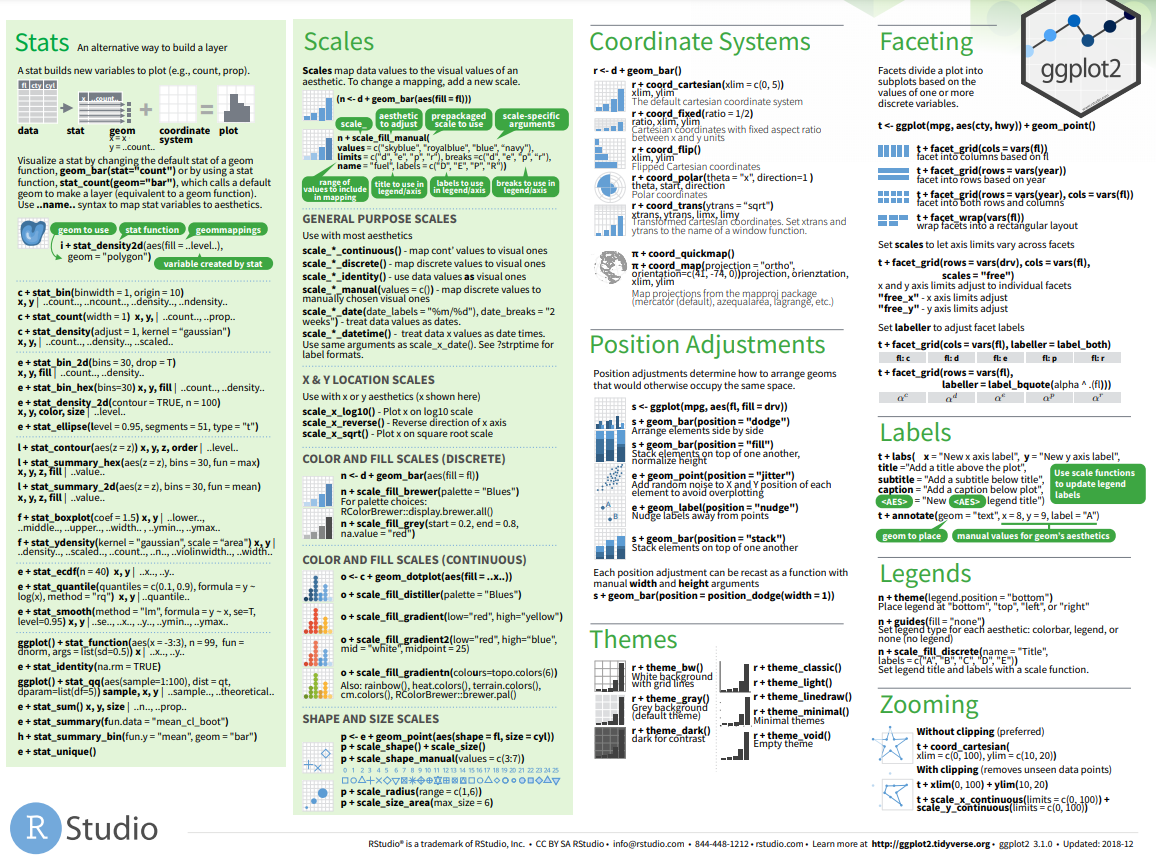
\includegraphics{images/ggplot cheat sheet 2.png}\\

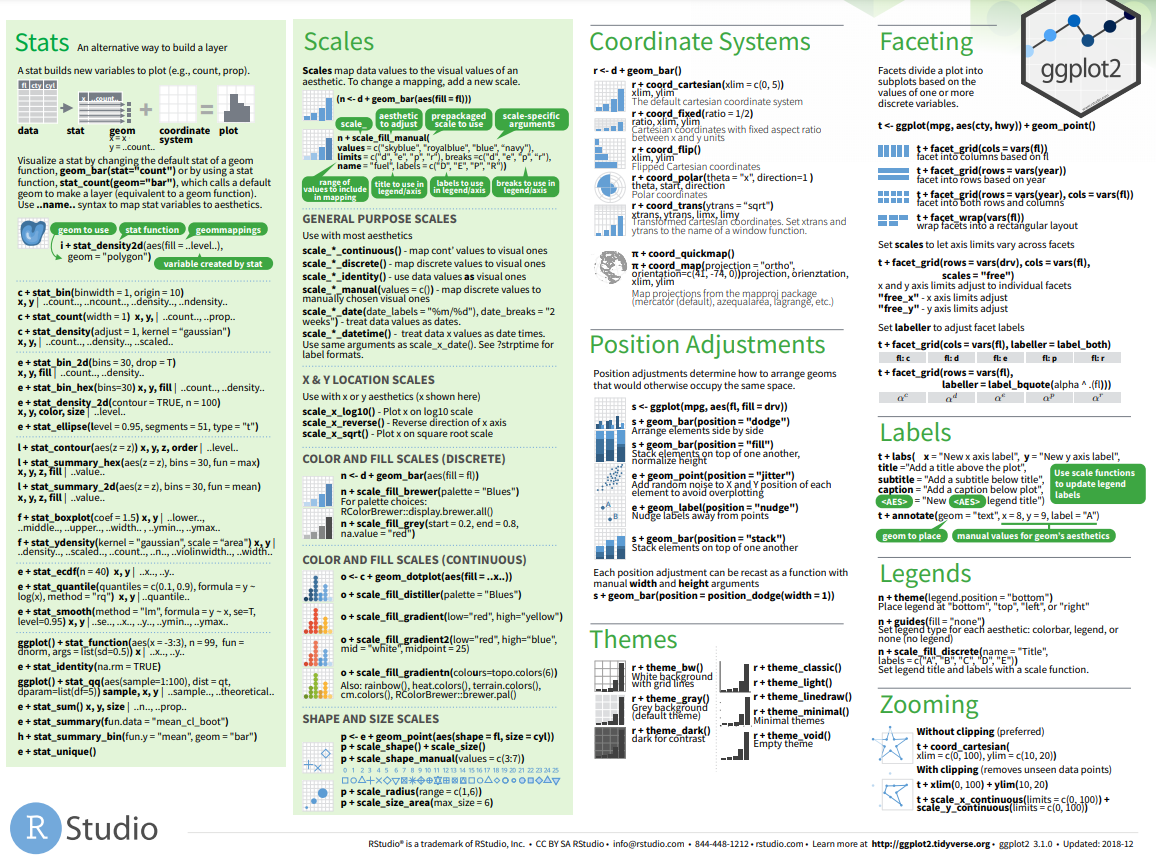
\includegraphics{images/ggplot cheat sheet 2.png}\\

\subsection{\texorpdfstring{\textbf{ggplot()}}{ggplot()}}

The ggplot() function is the base of the ggplot2 package. Using it
creates the space that we use to build a graph. If we run just the
ggplot() function we will get a gray rectangle. This is the space (and
background) of our plot!

\begin{Shaded}
\begin{Highlighting}[]
\FunctionTok{ggplot}\NormalTok{()}
\end{Highlighting}
\end{Shaded}

\begin{figure}[H]

{\centering 
\includegraphics{basic_graphs_files/figure-pdf/unnamed-chunk-2-1.pdf}

}

\end{figure}

To build a plot on the background, we must add to the ggplot call.
First, we need to tell it what data to use. Next, we need to tell it
where in the data frame to pull data from to build the axes and data
points. The part of the ggplot() function we use to build a graph is
called aes() or aesthetics.

Here is an example using penguins: I am telling ggplot that the data we
are using is `penguins' and then defining the x and y axis in the aes()
call with column names from penguins

\begin{Shaded}
\begin{Highlighting}[]
\FunctionTok{head}\NormalTok{(penguins)}
\end{Highlighting}
\end{Shaded}

\begin{verbatim}
# A tibble: 6 x 8
  species island    bill_length_mm bill_depth_mm flipper_l~1 body_~2 sex    year
  <fct>   <fct>              <dbl>         <dbl>       <int>   <int> <fct> <int>
1 Adelie  Torgersen           39.1          18.7         181    3750 male   2007
2 Adelie  Torgersen           39.5          17.4         186    3800 fema~  2007
3 Adelie  Torgersen           40.3          18           195    3250 fema~  2007
4 Adelie  Torgersen           NA            NA            NA      NA <NA>   2007
5 Adelie  Torgersen           36.7          19.3         193    3450 fema~  2007
6 Adelie  Torgersen           39.3          20.6         190    3650 male   2007
# ... with abbreviated variable names 1: flipper_length_mm, 2: body_mass_g
\end{verbatim}

\begin{Shaded}
\begin{Highlighting}[]
\FunctionTok{ggplot}\NormalTok{(}\AttributeTok{data=}\NormalTok{penguins, }\FunctionTok{aes}\NormalTok{(}\AttributeTok{x=}\NormalTok{species, }\AttributeTok{y=}\NormalTok{ bill\_length\_mm)) }
\end{Highlighting}
\end{Shaded}

\begin{figure}[H]

{\centering 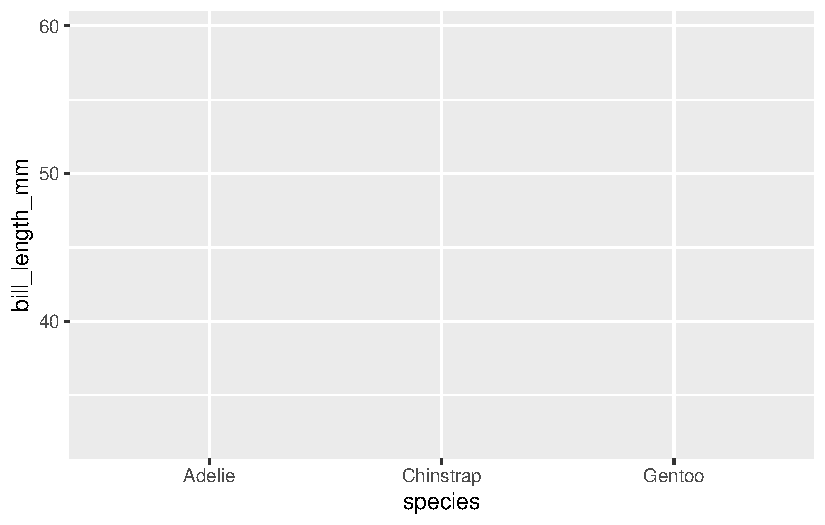
\includegraphics{basic_graphs_files/figure-pdf/unnamed-chunk-3-1.pdf}

}

\end{figure}

Like anything in R, we can give our plot a name and call it later

\begin{Shaded}
\begin{Highlighting}[]
\NormalTok{plot1}\OtherTok{\textless{}{-}}\FunctionTok{ggplot}\NormalTok{(}\AttributeTok{data=}\NormalTok{penguins, }\FunctionTok{aes}\NormalTok{(}\AttributeTok{x=}\NormalTok{species, }\AttributeTok{y=}\NormalTok{ bill\_length\_mm)) }

\NormalTok{plot1}
\end{Highlighting}
\end{Shaded}

\begin{figure}[H]

{\centering 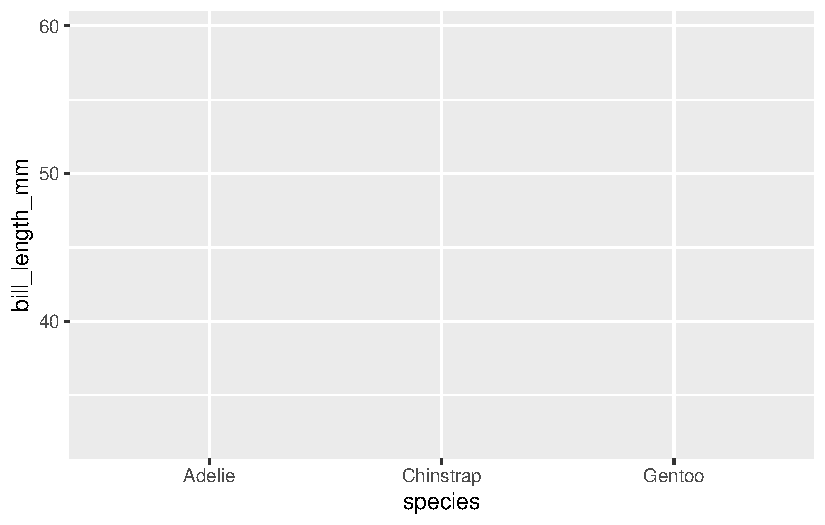
\includegraphics{basic_graphs_files/figure-pdf/unnamed-chunk-4-1.pdf}

}

\end{figure}

This is incredibly useful in ggplot as we can essentially add pieces to
make a more complete graph

\begin{Shaded}
\begin{Highlighting}[]
\NormalTok{plot1}\SpecialCharTok{+}
  \FunctionTok{geom\_boxplot}\NormalTok{()}\SpecialCharTok{+}
  \FunctionTok{geom\_point}\NormalTok{()}\SpecialCharTok{+}
  \FunctionTok{theme\_bw}\NormalTok{()}
\end{Highlighting}
\end{Shaded}

\begin{verbatim}
Warning: Removed 2 rows containing non-finite values (`stat_boxplot()`).
\end{verbatim}

\begin{verbatim}
Warning: Removed 2 rows containing missing values (`geom_point()`).
\end{verbatim}

\begin{figure}[H]

{\centering 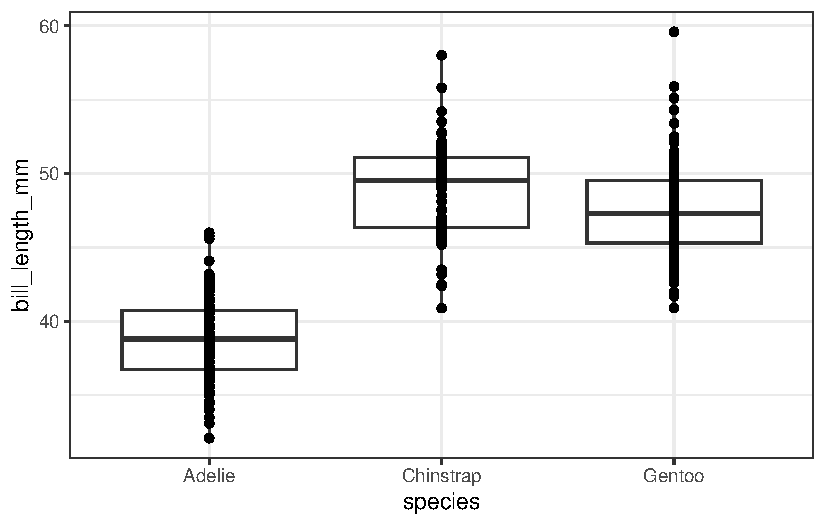
\includegraphics{basic_graphs_files/figure-pdf/unnamed-chunk-5-1.pdf}

}

\end{figure}

Before we get too excited about making perfect graphs, let's take a look
at the types of graphs we have available to us\ldots{}

\begin{center}\rule{0.5\linewidth}{0.5pt}\end{center}

\subsection{\texorpdfstring{\textbf{histogram}}{histogram}}

Histograms are used to explore the frequency distribution of a single
variable. We can check for normality (a bell curve) using this feature.
We can also look for means, skewed data, and other trends.

\begin{Shaded}
\begin{Highlighting}[]
\FunctionTok{ggplot}\NormalTok{(}\AttributeTok{data=}\NormalTok{penguins, }\FunctionTok{aes}\NormalTok{(bill\_length\_mm))}\SpecialCharTok{+}
  \FunctionTok{geom\_histogram}\NormalTok{()}
\end{Highlighting}
\end{Shaded}

\begin{verbatim}
`stat_bin()` using `bins = 30`. Pick better value with `binwidth`.
\end{verbatim}

\begin{verbatim}
Warning: Removed 2 rows containing non-finite values (`stat_bin()`).
\end{verbatim}

\begin{figure}[H]

{\centering 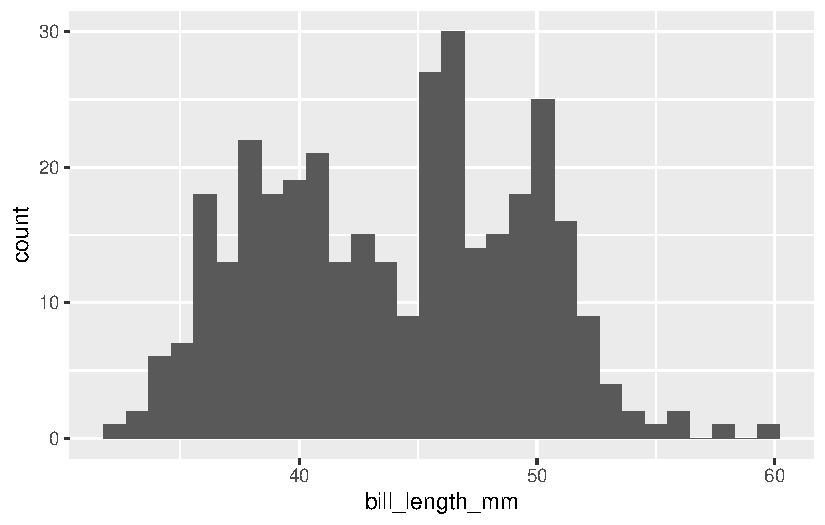
\includegraphics{basic_graphs_files/figure-pdf/unnamed-chunk-6-1.pdf}

}

\end{figure}

Within geom\_histogram we can use bin\_width to change the width of our
x-axis groupings.

\begin{Shaded}
\begin{Highlighting}[]
\FunctionTok{ggplot}\NormalTok{(}\AttributeTok{data=}\NormalTok{penguins, }\FunctionTok{aes}\NormalTok{(bill\_length\_mm))}\SpecialCharTok{+}
  \FunctionTok{geom\_histogram}\NormalTok{(}\AttributeTok{binwidth=}\DecValTok{5}\NormalTok{)}
\end{Highlighting}
\end{Shaded}

\begin{verbatim}
Warning: Removed 2 rows containing non-finite values (`stat_bin()`).
\end{verbatim}

\begin{figure}[H]

{\centering 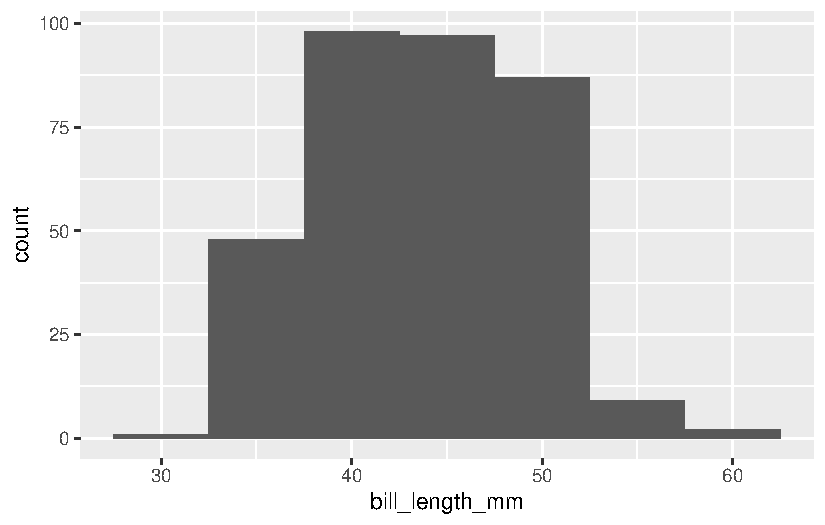
\includegraphics{basic_graphs_files/figure-pdf/unnamed-chunk-7-1.pdf}

}

\end{figure}

\subsection{\texorpdfstring{\textbf{boxplot}}{boxplot}}

A boxplot is a really useful plot to assess median and range of data. It
can also identify outliers! The defaults for a boxplot in ggplot produce
a median and interquartile range (IQR). The 1st quartile is the bottom
of the box and the 3rd quartile is the top. The whiskers show the spread
of the data where the ends of the whiskers represent the data points
that are the furthest from the median in either direction. Notably, if a
data point is 1.5 * IQR from the box (either the 1st or 3rd quartile) it
is an outlier. Outliers are excluded from whiskers and are presented as
points. There

Here's an example

\begin{Shaded}
\begin{Highlighting}[]
\FunctionTok{ggplot}\NormalTok{(}\AttributeTok{data=}\NormalTok{penguins, }\FunctionTok{aes}\NormalTok{(}\AttributeTok{x=}\NormalTok{species, }\AttributeTok{y=}\NormalTok{ bill\_length\_mm)) }\SpecialCharTok{+}
  \FunctionTok{geom\_boxplot}\NormalTok{()}
\end{Highlighting}
\end{Shaded}

\begin{verbatim}
Warning: Removed 2 rows containing non-finite values (`stat_boxplot()`).
\end{verbatim}

\begin{figure}[H]

{\centering 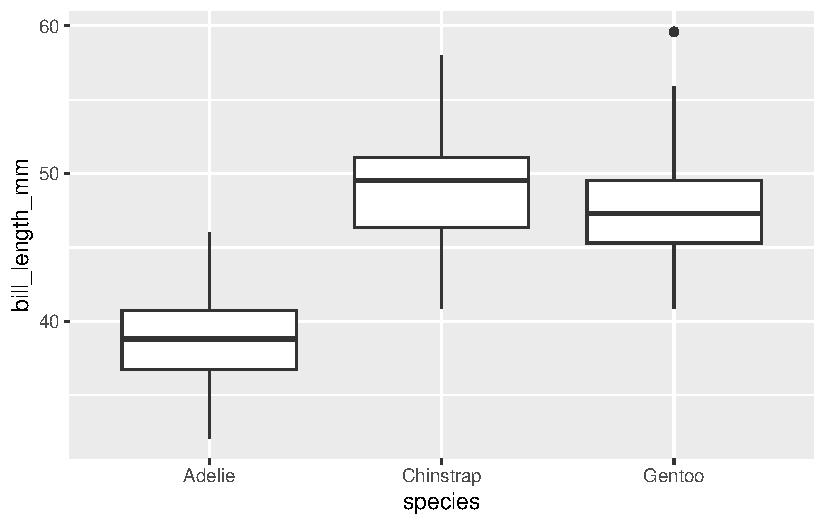
\includegraphics{basic_graphs_files/figure-pdf/unnamed-chunk-8-1.pdf}

}

\end{figure}

We can use geom\_violin to combine boxplot with a density plot (similar
to a histogram) Here we can see the distribution of values within bill
length by species.

\begin{Shaded}
\begin{Highlighting}[]
\FunctionTok{ggplot}\NormalTok{(}\AttributeTok{data=}\NormalTok{penguins, }\FunctionTok{aes}\NormalTok{(}\AttributeTok{x=}\NormalTok{species, }\AttributeTok{y=}\NormalTok{ bill\_length\_mm)) }\SpecialCharTok{+}
  \CommentTok{\#geom\_boxplot()+}
  \FunctionTok{geom\_violin}\NormalTok{()}
\end{Highlighting}
\end{Shaded}

\begin{verbatim}
Warning: Removed 2 rows containing non-finite values (`stat_ydensity()`).
\end{verbatim}

\begin{figure}[H]

{\centering 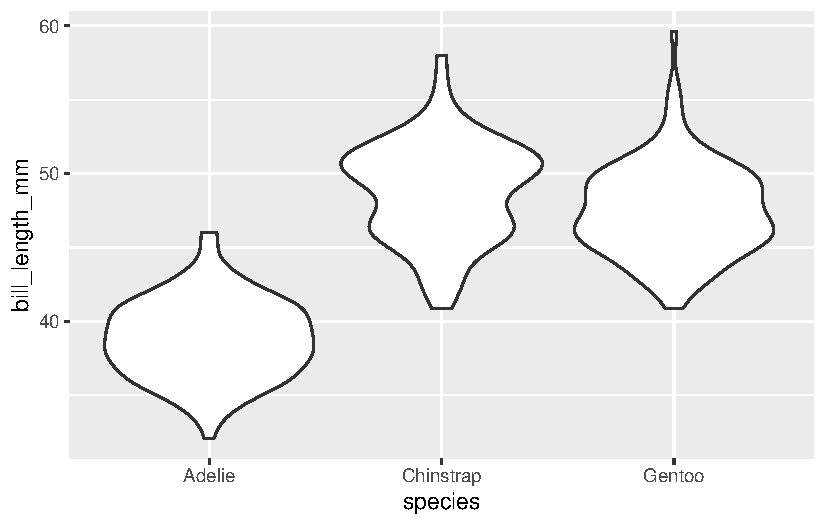
\includegraphics{basic_graphs_files/figure-pdf/unnamed-chunk-9-1.pdf}

}

\end{figure}

\begin{center}\rule{0.5\linewidth}{0.5pt}\end{center}

\subsection{\texorpdfstring{\textbf{bar graph}}{bar graph}}

We can make bar graphs in ggplot using geom\_bar(). There are some
tricks to getting bar graphs to work exactly right, which I will try to
detail below. \textbf{NOTE} Bar graphs are very rarely useful. If we
want to show means, why not just use points + error bars? What does the
bar actually represent? There aren't that many cases where we really
need bar graphs. There are exceptions, like when we have a population
and we want to see the demographics of that population by count or
percentage (see example below)

Here is a simple bar chart.

\begin{Shaded}
\begin{Highlighting}[]
\FunctionTok{ggplot}\NormalTok{(}\AttributeTok{data=}\NormalTok{penguins, }\FunctionTok{aes}\NormalTok{(species)) }\SpecialCharTok{+}
  \FunctionTok{geom\_bar}\NormalTok{()}
\end{Highlighting}
\end{Shaded}

\begin{figure}[H]

{\centering 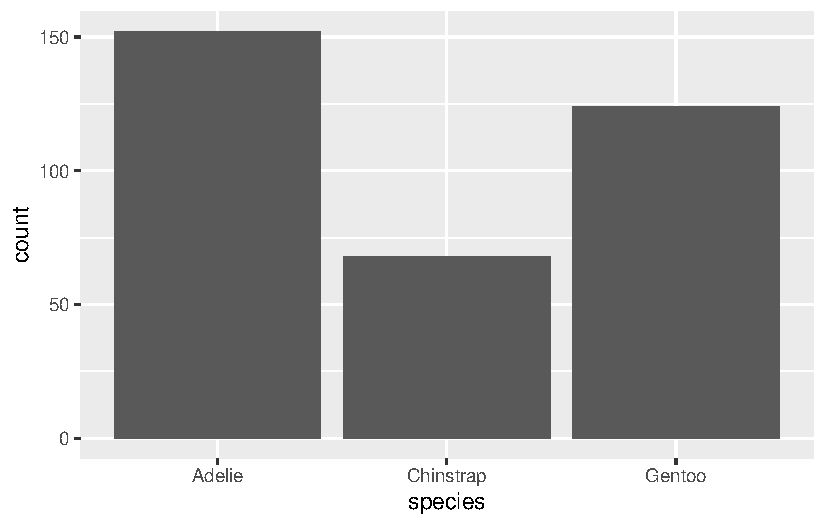
\includegraphics{basic_graphs_files/figure-pdf/unnamed-chunk-10-1.pdf}

}

\end{figure}

Here is a more elaborate boxplot that shows species breakdown by island!
Note that we use an aes() call within geom\_bar to define a fill. That
means fill by species, or add a color for each species.

\begin{Shaded}
\begin{Highlighting}[]
\FunctionTok{ggplot}\NormalTok{(}\AttributeTok{data=}\NormalTok{penguins, }\FunctionTok{aes}\NormalTok{(island)) }\SpecialCharTok{+}
  \FunctionTok{geom\_bar}\NormalTok{(}\FunctionTok{aes}\NormalTok{(}\AttributeTok{fill=}\NormalTok{species))}
\end{Highlighting}
\end{Shaded}

\begin{figure}[H]

{\centering 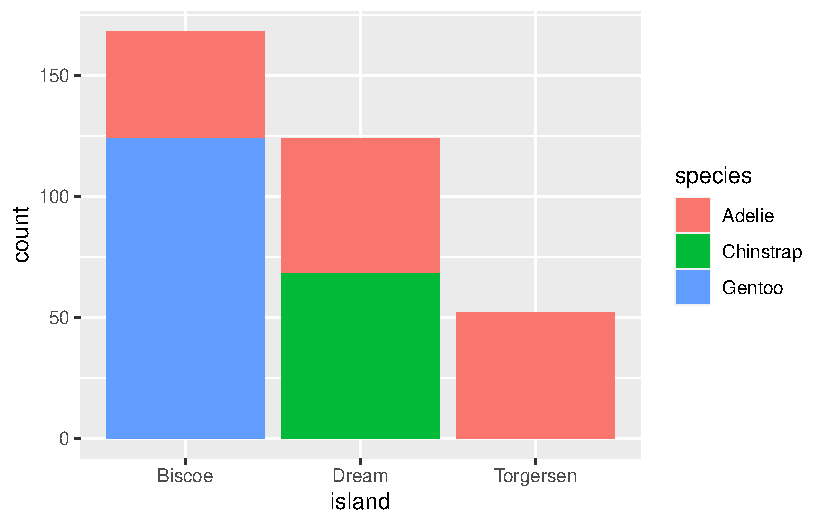
\includegraphics{basic_graphs_files/figure-pdf/unnamed-chunk-11-1.pdf}

}

\end{figure}

And here is that same plot with the bars unstacked. Instead of stacking,
we have used ``dodged'' each color to be its own bar.

\begin{Shaded}
\begin{Highlighting}[]
\FunctionTok{ggplot}\NormalTok{(}\AttributeTok{data=}\NormalTok{penguins, }\FunctionTok{aes}\NormalTok{(island)) }\SpecialCharTok{+}
  \FunctionTok{geom\_bar}\NormalTok{(}\FunctionTok{aes}\NormalTok{(}\AttributeTok{fill=}\NormalTok{species), }\AttributeTok{position=} \FunctionTok{position\_dodge}\NormalTok{())}
\end{Highlighting}
\end{Shaded}

\begin{figure}[H]

{\centering 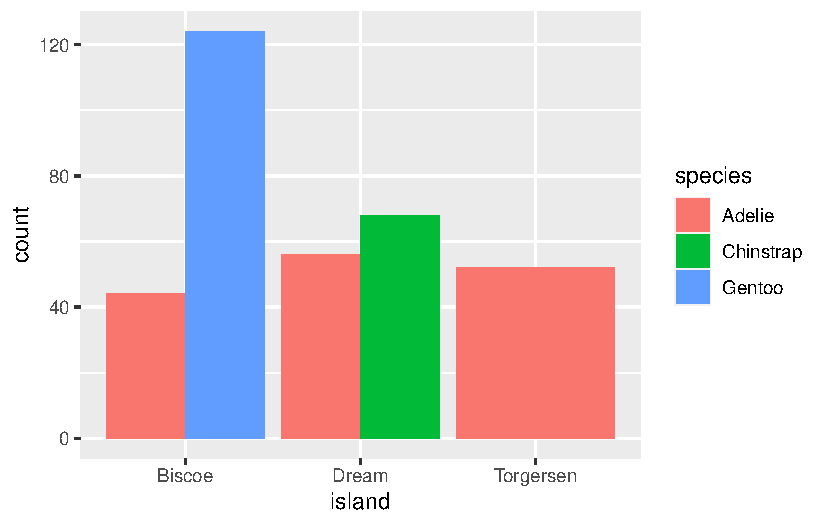
\includegraphics{basic_graphs_files/figure-pdf/unnamed-chunk-12-1.pdf}

}

\end{figure}

We learned when the best (only) times to use bar graphs are. Do you
remember what those were? Are the examples above representative of that?

\begin{center}\rule{0.5\linewidth}{0.5pt}\end{center}

\subsection{\texorpdfstring{\textbf{line graph}}{line graph}}

A line graph can be extremely useful, especially if we are looking at
time series data or rates!

Here is an example of CO2 uptake vs concentration in plants. Each color
represents a different plant. NOTE: the dataset called `CO2' is built
into R, so we can just use it without loading anything :)

\begin{Shaded}
\begin{Highlighting}[]
\FunctionTok{head}\NormalTok{(CO2)}
\end{Highlighting}
\end{Shaded}

\begin{verbatim}
  Plant   Type  Treatment conc uptake
1   Qn1 Quebec nonchilled   95   16.0
2   Qn1 Quebec nonchilled  175   30.4
3   Qn1 Quebec nonchilled  250   34.8
4   Qn1 Quebec nonchilled  350   37.2
5   Qn1 Quebec nonchilled  500   35.3
6   Qn1 Quebec nonchilled  675   39.2
\end{verbatim}

\begin{Shaded}
\begin{Highlighting}[]
\FunctionTok{ggplot}\NormalTok{(}\AttributeTok{data=}\NormalTok{CO2, }\FunctionTok{aes}\NormalTok{(}\AttributeTok{x=}\NormalTok{conc, }\AttributeTok{y=}\NormalTok{ uptake, }\AttributeTok{color=}\NormalTok{Plant)) }\SpecialCharTok{+}
  \FunctionTok{geom\_line}\NormalTok{()}
\end{Highlighting}
\end{Shaded}

\begin{figure}[H]

{\centering 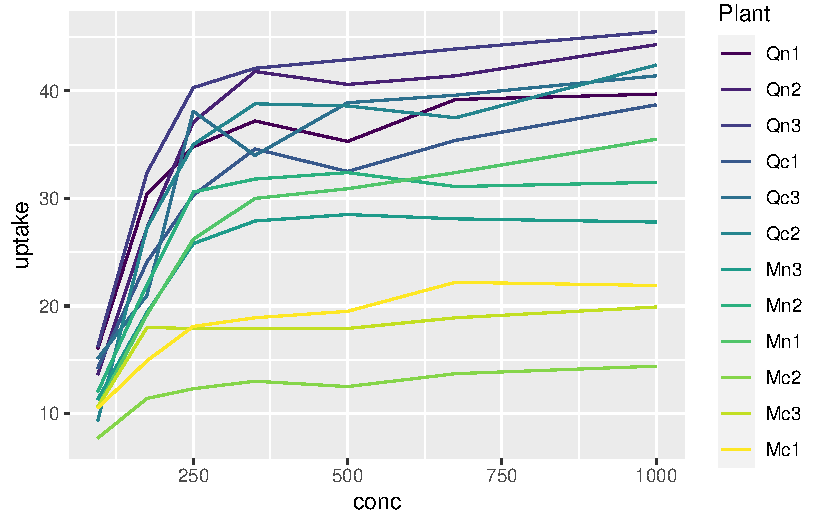
\includegraphics{basic_graphs_files/figure-pdf/unnamed-chunk-13-1.pdf}

}

\end{figure}

We can change the aesthetics of the lines using color, linetype, size,
etc. Here I am changing the linetype based on the plant species and
increasing the size of ALL lines to 2. This is a good example of how
aes() works. Anything within the aes() call is conditional. That means,
I give it a name (such as a column or variable name) and it changes
based on that column or variable. To change an aesthetic across all
lines, points, etc, I just put the code outside of the aes(). As I did
for size. That makes the size of ALL lines = 2.

\begin{Shaded}
\begin{Highlighting}[]
\FunctionTok{ggplot}\NormalTok{(}\AttributeTok{data=}\NormalTok{CO2, }\FunctionTok{aes}\NormalTok{(}\AttributeTok{x=}\NormalTok{conc, }\AttributeTok{y=}\NormalTok{ uptake, }\AttributeTok{color=}\NormalTok{Plant)) }\SpecialCharTok{+}
  \FunctionTok{geom\_line}\NormalTok{(}\FunctionTok{aes}\NormalTok{(}\AttributeTok{linetype=}\NormalTok{Plant),}\AttributeTok{size=}\DecValTok{2}\NormalTok{)}
\end{Highlighting}
\end{Shaded}

\begin{verbatim}
Warning: Using `size` aesthetic for lines was deprecated in ggplot2 3.4.0.
i Please use `linewidth` instead.
\end{verbatim}

\begin{figure}[H]

{\centering 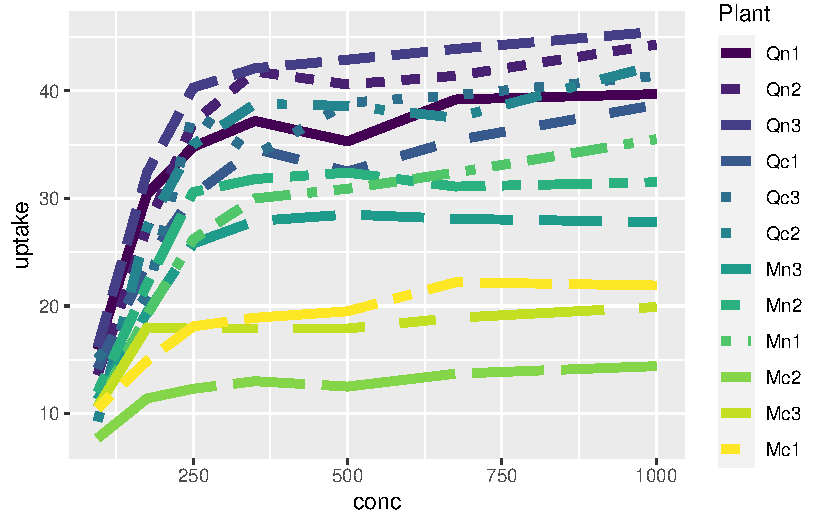
\includegraphics{basic_graphs_files/figure-pdf/unnamed-chunk-14-1.pdf}

}

\end{figure}

\begin{center}\rule{0.5\linewidth}{0.5pt}\end{center}

\subsection{\texorpdfstring{\textbf{scatter plot}}{scatter plot}}

The scatter plot is probably the most commonly used graphical tool in
ggplot. It is based on the geom\_point() function

\begin{Shaded}
\begin{Highlighting}[]
\FunctionTok{ggplot}\NormalTok{(}\AttributeTok{data=}\NormalTok{penguins, }\FunctionTok{aes}\NormalTok{(}\AttributeTok{x=}\NormalTok{species, }\AttributeTok{y=}\NormalTok{ bill\_length\_mm)) }\SpecialCharTok{+}
  \FunctionTok{geom\_point}\NormalTok{()}
\end{Highlighting}
\end{Shaded}

\begin{verbatim}
Warning: Removed 2 rows containing missing values (`geom_point()`).
\end{verbatim}

\begin{figure}[H]

{\centering 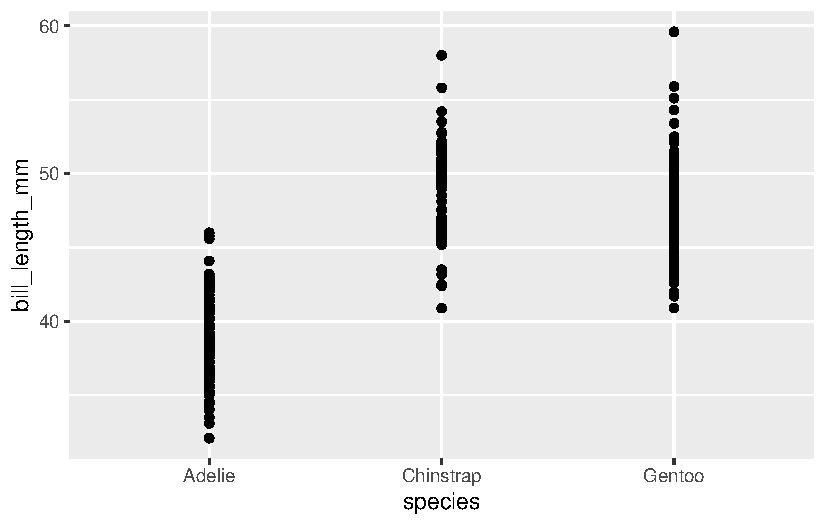
\includegraphics{basic_graphs_files/figure-pdf/unnamed-chunk-15-1.pdf}

}

\end{figure}

Importantly, we can use the data= and aes() calls within geom\_point()
or any other geom instead of within ggplot() if needed. Why might this
be important?

\begin{Shaded}
\begin{Highlighting}[]
\FunctionTok{ggplot}\NormalTok{() }\SpecialCharTok{+}
  \FunctionTok{geom\_point}\NormalTok{(}\AttributeTok{data=}\NormalTok{penguins, }\FunctionTok{aes}\NormalTok{(}\AttributeTok{x=}\NormalTok{species, }\AttributeTok{y=}\NormalTok{ bill\_length\_mm))}
\end{Highlighting}
\end{Shaded}

\begin{verbatim}
Warning: Removed 2 rows containing missing values (`geom_point()`).
\end{verbatim}

\begin{figure}[H]

{\centering 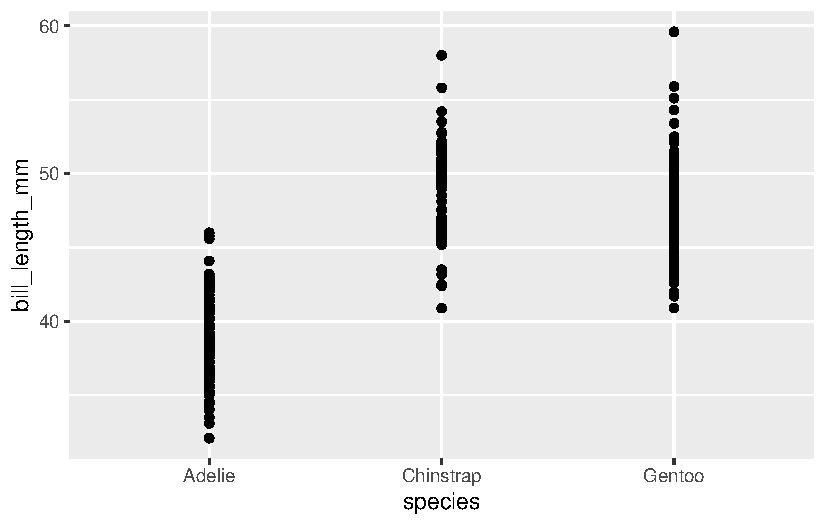
\includegraphics{basic_graphs_files/figure-pdf/unnamed-chunk-16-1.pdf}

}

\end{figure}

Sometimes we don't want to plot all of our points on the same vertical
line. If that is the case, we can use geom\_jitter()

\begin{Shaded}
\begin{Highlighting}[]
\FunctionTok{ggplot}\NormalTok{(}\AttributeTok{data=}\NormalTok{penguins, }\FunctionTok{aes}\NormalTok{(}\AttributeTok{x=}\NormalTok{species, }\AttributeTok{y=}\NormalTok{ bill\_length\_mm)) }\SpecialCharTok{+}
  \FunctionTok{geom\_jitter}\NormalTok{()}
\end{Highlighting}
\end{Shaded}

\begin{verbatim}
Warning: Removed 2 rows containing missing values (`geom_point()`).
\end{verbatim}

\begin{figure}[H]

{\centering 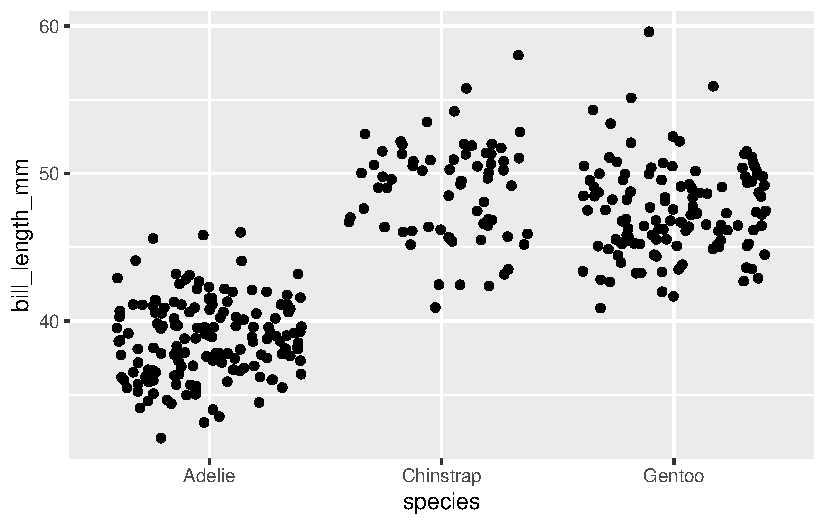
\includegraphics{basic_graphs_files/figure-pdf/unnamed-chunk-17-1.pdf}

}

\end{figure}

\begin{center}\rule{0.5\linewidth}{0.5pt}\end{center}

\subsection{\texorpdfstring{\textbf{Adding error
bars}}{Adding error bars}}

We often want to present means and error in our visualizations. This can
be done through the use of geom\_boxplot() or through combining
geom\_point() with geom\_errorbar()

Here is an example of the later\ldots{}

\begin{Shaded}
\begin{Highlighting}[]
\CommentTok{\#First, we need to calculate a mean bill length for our penguins by species and island}
\NormalTok{sumpens}\OtherTok{\textless{}{-}}\NormalTok{ penguins }\SpecialCharTok{\%\textgreater{}\%}
  \FunctionTok{group\_by}\NormalTok{(species, island) }\SpecialCharTok{\%\textgreater{}\%}
  \FunctionTok{na.omit}\NormalTok{() }\SpecialCharTok{\%\textgreater{}\%} \CommentTok{\#removes rows with NA values (a few rows may otherwise have NA due to sampling error in the field)}
  \FunctionTok{summarize}\NormalTok{(}\AttributeTok{meanbill=}\FunctionTok{mean}\NormalTok{(bill\_length\_mm), }\AttributeTok{sd=}\FunctionTok{sd}\NormalTok{(bill\_length\_mm), }\AttributeTok{n=}\FunctionTok{n}\NormalTok{(), }\AttributeTok{se=}\NormalTok{sd}\SpecialCharTok{/}\FunctionTok{sqrt}\NormalTok{(n))}

\NormalTok{sumpens}
\end{Highlighting}
\end{Shaded}

\begin{verbatim}
# A tibble: 5 x 6
# Groups:   species [3]
  species   island    meanbill    sd     n    se
  <fct>     <fct>        <dbl> <dbl> <int> <dbl>
1 Adelie    Biscoe        39.0  2.48    44 0.374
2 Adelie    Dream         38.5  2.48    55 0.335
3 Adelie    Torgersen     39.0  3.03    47 0.442
4 Chinstrap Dream         48.8  3.34    68 0.405
5 Gentoo    Biscoe        47.6  3.11   119 0.285
\end{verbatim}

\begin{Shaded}
\begin{Highlighting}[]
\CommentTok{\# Now we can plot! }
\FunctionTok{ggplot}\NormalTok{(}\AttributeTok{data=}\NormalTok{sumpens, }\FunctionTok{aes}\NormalTok{(}\AttributeTok{x=}\NormalTok{species, }\AttributeTok{y=}\NormalTok{meanbill, }\AttributeTok{color=}\NormalTok{island))}\SpecialCharTok{+}
  \FunctionTok{geom\_point}\NormalTok{()}\SpecialCharTok{+}
  \FunctionTok{geom\_errorbar}\NormalTok{(}\AttributeTok{data=}\NormalTok{sumpens, }\FunctionTok{aes}\NormalTok{(}\AttributeTok{x=}\NormalTok{species, }\AttributeTok{ymin=}\NormalTok{meanbill}\SpecialCharTok{{-}}\NormalTok{se, }\AttributeTok{ymax=}\NormalTok{meanbill}\SpecialCharTok{+}\NormalTok{se), }\AttributeTok{width=}\FloatTok{0.2}\NormalTok{)}
\end{Highlighting}
\end{Shaded}

\begin{figure}[H]

{\centering 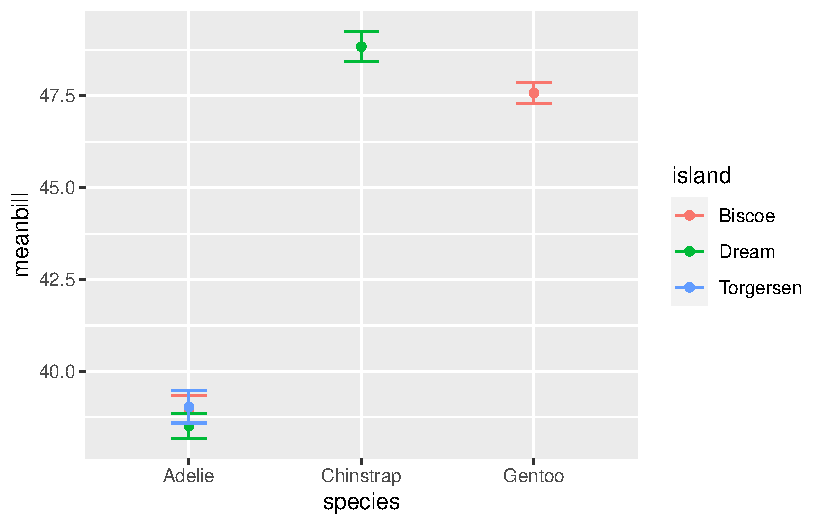
\includegraphics{basic_graphs_files/figure-pdf/unnamed-chunk-18-1.pdf}

}

\end{figure}

And if we want to be extra fancy (and rigorous), we can plot the raw
data behind the mean+error This is considered a \textbf{graphical best
practice} as we can see the mean, error, and the true spread of the
data!

\begin{Shaded}
\begin{Highlighting}[]
\FunctionTok{ggplot}\NormalTok{()}\SpecialCharTok{+}
  \FunctionTok{geom\_jitter}\NormalTok{(}\AttributeTok{data=}\NormalTok{ penguins, }\FunctionTok{aes}\NormalTok{(}\AttributeTok{x=}\NormalTok{species, }\AttributeTok{y=}\NormalTok{bill\_length\_mm, }\AttributeTok{color=}\NormalTok{island), }\AttributeTok{alpha=}\FloatTok{0.5}\NormalTok{, }\AttributeTok{width=}\FloatTok{0.2}\NormalTok{)}\SpecialCharTok{+} \CommentTok{\#this is the raw data}
  \FunctionTok{geom\_point}\NormalTok{(}\AttributeTok{data=}\NormalTok{sumpens, }\FunctionTok{aes}\NormalTok{(}\AttributeTok{x=}\NormalTok{species, }\AttributeTok{y=}\NormalTok{meanbill, }\AttributeTok{color=}\NormalTok{island), }\AttributeTok{size=}\DecValTok{3}\NormalTok{)}\SpecialCharTok{+} \CommentTok{\#this is the averages}
  \FunctionTok{geom\_errorbar}\NormalTok{(}\AttributeTok{data=}\NormalTok{sumpens, }\FunctionTok{aes}\NormalTok{(}\AttributeTok{x=}\NormalTok{species, }\AttributeTok{ymin=}\NormalTok{meanbill}\SpecialCharTok{{-}}\NormalTok{se, }\AttributeTok{ymax=}\NormalTok{meanbill}\SpecialCharTok{+}\NormalTok{se), }\AttributeTok{width=}\FloatTok{0.1}\NormalTok{)}
\end{Highlighting}
\end{Shaded}

\begin{verbatim}
Warning: Removed 2 rows containing missing values (`geom_point()`).
\end{verbatim}

\begin{figure}[H]

{\centering 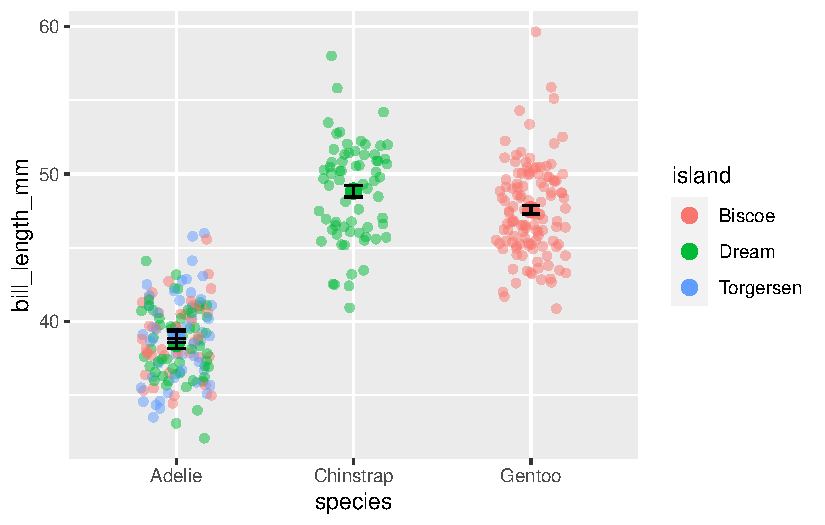
\includegraphics{basic_graphs_files/figure-pdf/unnamed-chunk-19-1.pdf}

}

\end{figure}

An alternative to geom\_jitter, which doesn't always work, is to use
geom\_point but force the points to not overlap with position\_dodge.
Here is an example

\begin{Shaded}
\begin{Highlighting}[]
\CommentTok{\#first we should define the distance of our position\_dodge}
\NormalTok{pd}\OtherTok{\textless{}{-}}\FunctionTok{position\_dodge}\NormalTok{(}\AttributeTok{width=}\FloatTok{0.2}\NormalTok{)}

\FunctionTok{ggplot}\NormalTok{(}\AttributeTok{data=}\NormalTok{sumpens, }\FunctionTok{aes}\NormalTok{(}\AttributeTok{x=}\NormalTok{species, }\AttributeTok{y=}\NormalTok{meanbill, }\AttributeTok{color=}\NormalTok{island))}\SpecialCharTok{+}
  \FunctionTok{geom\_point}\NormalTok{(}\AttributeTok{data=}\NormalTok{ penguins, }\FunctionTok{aes}\NormalTok{(}\AttributeTok{x=}\NormalTok{species, }\AttributeTok{y=}\NormalTok{bill\_length\_mm, }\AttributeTok{color=}\NormalTok{island), }\AttributeTok{alpha=}\FloatTok{0.2}\NormalTok{, }\AttributeTok{width=}\FloatTok{0.2}\NormalTok{, }\AttributeTok{position=}\NormalTok{pd)}\SpecialCharTok{+} \CommentTok{\#raw data}
  \FunctionTok{geom\_point}\NormalTok{(}\AttributeTok{size=}\DecValTok{3}\NormalTok{, }\AttributeTok{position=}\NormalTok{pd)}\SpecialCharTok{+} \CommentTok{\#averages}
  \FunctionTok{geom\_errorbar}\NormalTok{(}\FunctionTok{aes}\NormalTok{(}\AttributeTok{ymin=}\NormalTok{meanbill}\SpecialCharTok{{-}}\NormalTok{se, }\AttributeTok{ymax=}\NormalTok{meanbill}\SpecialCharTok{+}\NormalTok{se), }\AttributeTok{width=}\FloatTok{0.2}\NormalTok{, }\AttributeTok{position=}\NormalTok{pd)}
\end{Highlighting}
\end{Shaded}

\begin{verbatim}
Warning in geom_point(data = penguins, aes(x = species, y = bill_length_mm, :
Ignoring unknown parameters: `width`
\end{verbatim}

\begin{verbatim}
Warning: Removed 2 rows containing missing values (`geom_point()`).
\end{verbatim}

\begin{figure}[H]

{\centering 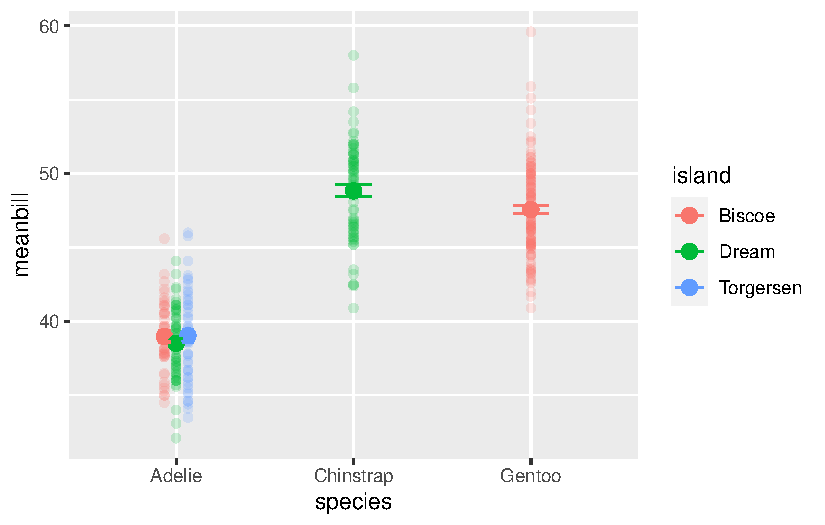
\includegraphics{basic_graphs_files/figure-pdf/unnamed-chunk-20-1.pdf}

}

\end{figure}

This code will produce the same graph as above. Note that in
geom\_jitter we just replaced width = with position =

\begin{Shaded}
\begin{Highlighting}[]
\FunctionTok{ggplot}\NormalTok{(sumpens, }\FunctionTok{aes}\NormalTok{(}\AttributeTok{x=}\NormalTok{species, }\AttributeTok{y=}\NormalTok{ meanbill, }\AttributeTok{color=}\NormalTok{island))}\SpecialCharTok{+}
  \FunctionTok{geom\_jitter}\NormalTok{(}\AttributeTok{data=}\NormalTok{ penguins, }\FunctionTok{aes}\NormalTok{(}\AttributeTok{x=}\NormalTok{species, }\AttributeTok{y=}\NormalTok{bill\_length\_mm, }\AttributeTok{color=}\NormalTok{island), }\AttributeTok{alpha=}\FloatTok{0.5}\NormalTok{, }\AttributeTok{position=}\NormalTok{pd)}\SpecialCharTok{+} \CommentTok{\#this is the raw data}
  \FunctionTok{geom\_point}\NormalTok{(}\AttributeTok{size=}\DecValTok{3}\NormalTok{,}\AttributeTok{position=}\NormalTok{pd)}\SpecialCharTok{+} \CommentTok{\#this is the averages}
  \FunctionTok{geom\_errorbar}\NormalTok{(}\FunctionTok{aes}\NormalTok{(}\AttributeTok{ymin=}\NormalTok{meanbill}\SpecialCharTok{{-}}\NormalTok{se, }\AttributeTok{ymax=}\NormalTok{meanbill}\SpecialCharTok{+}\NormalTok{se), }\AttributeTok{width=}\FloatTok{0.2}\NormalTok{, }\AttributeTok{position=}\NormalTok{pd)}
\end{Highlighting}
\end{Shaded}

\begin{verbatim}
Warning: Removed 2 rows containing missing values (`geom_point()`).
\end{verbatim}

\begin{figure}[H]

{\centering 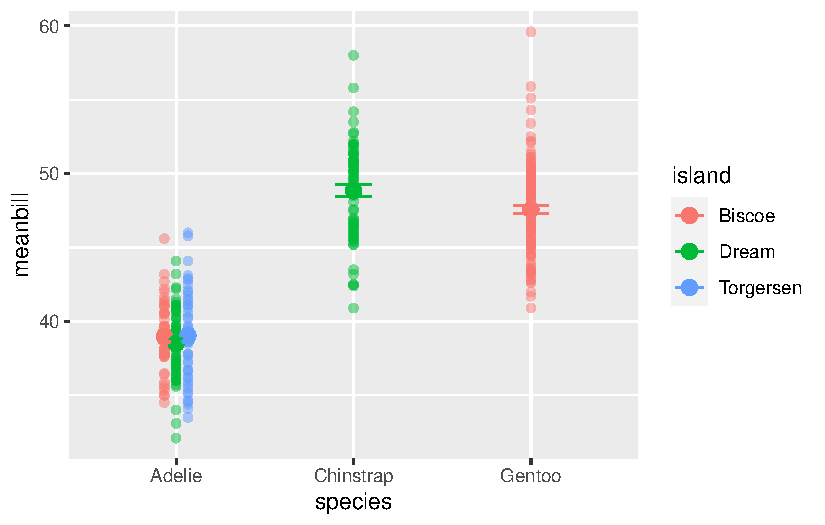
\includegraphics{basic_graphs_files/figure-pdf/unnamed-chunk-21-1.pdf}

}

\end{figure}

\begin{center}\rule{0.5\linewidth}{0.5pt}\end{center}



\end{document}
